\documentclass{article}
\usepackage{tikz, comment}
\usepackage{pifont}
\usepackage{fontspec, pgfplots}
\usetikzlibrary{arrows, decorations.markings, decorations.pathreplacing}
\begin{comment}
:Title: Not defined yet
:Tags: moment;focus of a parabola;median of a trapezoid;pappus&#146;s theorem, theorem of pappus;permutation
:Prob: 0.5708;0.5622;0.5572;0.5381;0.5375
:Author: Prof.Hu Ji-shan, HKUST
:Slug: No name yet

Description Here.........
\end{comment}
\begin{document}\centering 

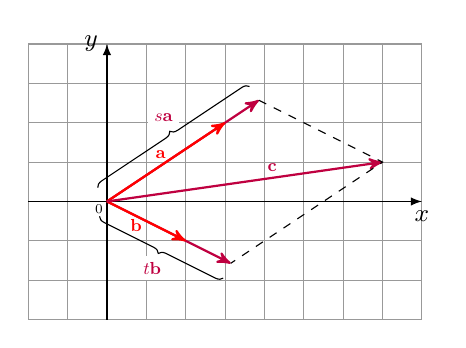
\begin{tikzpicture}[>=latex,xscale=.5*1, yscale=.5*1][font=\sf\small] 

\draw[xstep=1cm,ystep=1cm,color=gray!80] (-2, -3) grid (8, 4);

    	\foreach \x in {}
     		\draw (\x,2pt/8) -- (\x,-2pt/8)
			node[anchor=north] {\tiny$\x$}
			;

    	\foreach \x in {}
     		\draw (\x,2pt/1) -- (\x,-2pt/1)
			node[anchor=south] {\tiny$\x$}
			;
    	\foreach \y in {}
     		\draw (-2pt/1,\y) -- (2pt/1,\y)
			node[anchor=east] {\tiny $\y$}
			;

\draw[->] (-2, 0) -- (8, 0)node[below] {$x$} ;
\draw[->] (0, -3) -- (0, 4)node[left] {$y$} ;

\draw[purple, thick, ->, >=stealth'] (0, 0) -- ({3*9/7}, {2*9/7});

\draw [decoration={brace,raise=6},decorate, xshift=0] 
(0, 0) -- ({3*9/7}, {2*9/7})node[purple, fill=white, midway, pos=0.5, xshift=-7, yshift=12, scale=0.7]{$s{\bf a}$};

\draw[red, thick, opacity=1, ->, >=stealth'] (0, 0) -- (3, 2)node[opacity=1, left, midway, pos=0.6, xshift=-2, yshift=0, scale=0.7]{${\bf a}$};

\draw[purple, thick, ->, >=stealth'] (0, 0) -- ({2*11/7}, {-1*11/7});

\draw [decoration={brace,raise=6, mirror},decorate, xshift=0] 
(0, 0) -- ({2*11/7}, {-1*11/7})node[purple, fill=white, midway, pos=0.5, xshift=-6, yshift=-13, scale=0.7]{$t{\bf b}$};

\draw[red, thick, ->, >=stealth'] (0, 0) -- (2, -1)node[opacity=1, left, midway, pos=0.6, xshift=-2, yshift=0, scale=0.7]{${\bf b}$};

\draw[purple, thick, ->, >=stealth'] (0, 0) -- (7, 1)node[above, midway, pos=0.6, xshift=0, yshift=0, scale=0.7]{${\bf c}$};

\draw[dashed] ({3*9/7}, {2*9/7})--(7, 1)--({2*11/7}, {-1*11/7});

\node[scale=0.7] at (-0.2/1, -0.2/1) {\scriptsize$0$};

\end{tikzpicture}
\end{document}